\chapter{Analisis dan Perancangan}
\label{Analisis dan Perancangan}

Pada bab ini akan dibahas mengenai dan perancangan program. Bagian dari analisis terdiri dari
analisis set data, analisis masukan dan keluaran, serta analisis output. Analisis yang akan dilakukan berupa aliran \textit{log web} dan twitter.

\section{Analisis dan Perancangan Penghitung Hashtag pada Data Stream Twitter}
Perangkat lunak yang akan dikembangakan adalah perangkat lunak spark. Perangkat lunak digunakan untuk mengambil data dengan sistem \textit{spark streaming} dan melakukan analisis sederhana secara \textit{real-time}. Program saat ini akan menghitung jumlah hashtag terbanyak pada lima menit terakhir.

\subsection{Analisis Set Data}
set data yang akan diambil oleh \textit{spark streaming} bersifat \textit{real-time}. Hal ini dilakukan dengan mengintegrasikan \textit{spark streaming} dengan sistem eksternal yang meyediakan data melalui API. Untuk kasus ini akan digunakan data yang berasal dari twitter.
 
\subsection{Analisis Masukan dan Keluaran}
Data yang didapatkan dari twitter adalah berupa \textit{twitter object} dalam format JSON. Data twitter akan diambil selama 5 menit dan keluaran akan berupa pasangan key value yang bernilai (hashtag,value).

\section{Perancangan Penghitung Hashtag}

Untuk membuat sistem penghitung hashtag bekerja, harus membuat batch window yang nanti akan diintegrasikan dengan Twitter. Lalu Setiap Objek akan dipetakan dan hanya diambil statusnya saja karena informasi hashtag terletak pada status seseorang. Status yang telah didapat akan dipetakan lagi dan dipisahkan perkata. Lalu fungsi filter akan dipanggil dan kita hanya mengambil simbol \# yang merepresentasikan \textit{Hashtag}. Hashtag akan dipetakan lagi dengan map hingga berisi pasangan key value. dengan nilai key adalah hashtag dan value adalah jumlahnya. Lalu akan dilakukan \textit{reduce} berdasarkan nilai key dan batch window yang sama. Atur ukuran window menjadi 5 menit.

		\begin{figure}[H] 
		\centering  
		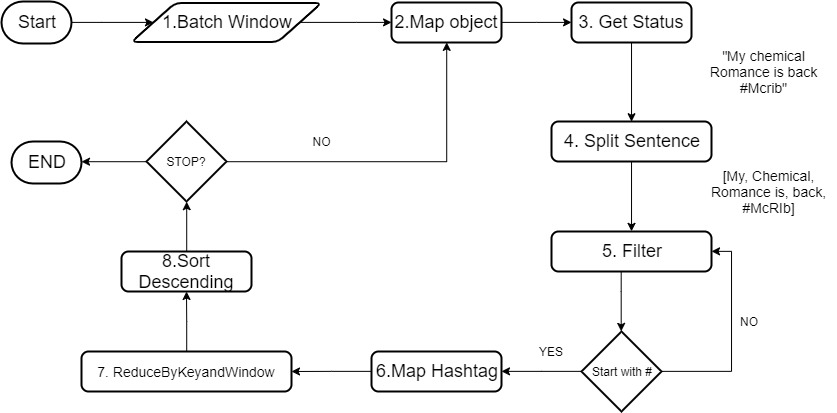
\includegraphics[scale=0.5]{HashtagFlow}  
		\caption[Twitter Obejct]{Flowchart diagram analisis hashtag} 
		\label{fig:processing-events relationship} 
		\end{figure}
		
\begin{enumerate}
		\item[1.]Membuat batch window berukuran satu detik. setiap satu detik akan menangkap
		objek-objek dari twitter.
		\item[2.]Memetakan setiap objek menjadi statusnya saja artinya dari seluruh objek tweet
		seperti nama atau location yang kita ambil hanya perkataan yang diposting oleh user 					saja.
		\item[3.]Mengambil statusnya satu per satu
		\item[4.]Membagi kalimat berdasarkan spasi lalu menyimpannya di array
		\item[5.]Filter setiap elemen pada array jika elemen pada array tidak sama
		dengan \# maka akan terus melakukan filter sampai status pada batch ini habis
		\item[6.]memetakan hashtag menjadi $[key,value] =>[hashtag,1]$
		\item[7.]melakukan reduce penjumlahan berdasarkan key dan windows yang sama.
		\item[8.]Mengurutkan hashtag berdasarkan value dari nilai yang paling tinggi.
		\item[9.]Jika program sudah diberhentikan maka tidak akan mengumpulkan objek lagi.
		Tetapi, jika tidak akan terus berlanjut.
\end{enumerate}